%% Mans Maģistrs
\documentclass[magjistrs]{vea-diplomdarbs}
\usepackage{setspace}	% Line spacing package
\usepackage{calc}

%% Use proper Aurora Bold Condensed BT
\definecolor{SeaBlue}{cmyk}{1,0,0.37,0.52}
\newfontfamily\TitleFont[%
	Path = /home/johnlm/Development/resources/tex_graphics_lib/fonts/ ,%
	FakeStretch = 1.5 ,
	Color = SeaBlue
	]{aurora-BT-condensed-bold}

\setotherlanguages{english,russian}

\newcommand{\TODO}{\textcolor{red}{TODO}}

%% Inline Word inclusion formatting
\newcommand{\termEn}[1]{\textenglish{\itshape {#1}}} % inline English
\newcommand{\termLatin}[1]{\textit{#1}} % inline Latin
\newcommand{\termTech}[1]{\textit{#1}} % technical term (LV?)
\newcommand{\newTerm}[1]{,,{#1}''} %newly mentioned term

%% Pāris matemātikas komandu definīcijas
\newcommand{\vb}[1]{\mathbf{#1}}

%% English determined number suffixes
\newcommand{\st}{\textsuperscript{st} }
\newcommand{\nd}{\textsuperscript{nd} }
\newcommand{\rd}{\textsuperscript{rd} }
\newcommand{\nth}{\textsuperscript{th} }

\hyphenpenalty=7500
\clubpenalty=9000
\widowpenalty=9000

\title{Attēlu raksturpunktu pāru noteikšanas algoritmu ātrdarbības izpēte dažādām aparatūras platformām}
\author{Jānis Šmēdiņš}

% Hyperref package for links in PDF (should be last package)
\usepackage[hyperfootnotes=false,linkbordercolor={blue},hyperindex]{hyperref}
\hypersetup{pdftitle={Attēlu raksturpunktu pāru noteikšanas algoritmu ātrdarbības izpēte dažādām aparatūras platformām}}
\hypersetup{pdfauthor={Jānis Šmēdiņš}}
\usepackage{fixlatvian}

\begin{document}
	% Titullapa
	\pagestyle{empty}
	% LM izcilā VeA titullapa bakalauram!
\begin{titlepage}
	% VeA Logo
	% "Ventspils Austskola" virsraksts (\TitleFont jābūt definētam!!!)
	\newsavebox{\veatext}
	\savebox{\veatext}{
		\TitleFont\Huge\MakeUppercase{Ventspils Augstskola}}
	% Teksta platuma noteikšana (lai pielīdzinātu bildi tā platumam}
	\newlength{\veatextwidth}
	\settowidth{\veatextwidth}{\usebox{\veatext}}
	% Šeit drukāts pats logo un nosaukums
	\centering
\includegraphics[width=0.98\veatextwidth]{VeA_logo.pdf}\\[4pt]
	\usebox{\veatext}\\[6pt]
	\large Informācijas tehnoloģiju fakultāte\\[2cm]
	
	%\textbf{Maģistra darbs}\\[1.5cm]
	\textbf{Maģistra darba 1.~atskaite}\\[1.5cm]
	
	\textsc{\Large Attēlu raksturpunktu atrašanas un salāgošanas algoritmu veiktspējas izpēte uz dažādām aparatūras platformām}
	\vfill % LIELĀ atstarpe
	
	%\raggedleft
	\normalsize
	\begin{minipage}[t]{0.3\textwidth}
		\begin{flushleft}
			Autors
		\end{flushleft}
	\end{minipage}
	\begin{minipage}[t]{0.65\textwidth}
		\begin{flushleft}
			Ventspils Augstskolas \\
			Informācijas tehnoloģiju fakultātes \\
			profesionālās maģistra studiju programmas „Elektronika”\\
			2.~kursa students \\
			\textbf{Jānis Šmēdiņš}\\
			Matr.~nr.~\texttt{12140012}\\
			\rule[-1em]{10em}{1pt}\\
			\makebox[10em][c]{\tiny (paraksts)}\\[1cm]
		\end{flushleft}
	\end{minipage}\\[2em]
	\begin{minipage}[t]{0.3\textwidth}
		\begin{flushleft}
			Fakultātes dekāns
		\end{flushleft}
	\end{minipage}
	\begin{minipage}[t]{0.65\textwidth}
		\begin{flushleft}
			asoc.prof.,~Dr.~math.~Gaļina Hiļķeviča\\[1ex]
			\rule[-1em]{10em}{1pt}\\
			\makebox[10em][c]{\tiny (paraksts)}\\[1cm]
		\end{flushleft}
	\end{minipage}\\[2em]
	\begin{minipage}[t]{0.3\textwidth}
		\begin{flushleft}
			Zinātniskais vadītājs
		\end{flushleft}
	\end{minipage}
	\begin{minipage}[t]{0.65\textwidth}
		\begin{flushleft}
			pētnieks, Dr.~sc.~comp.~Kaspars Sudars\\[1ex]
			\rule[-1em]{10em}{1pt}\\
			\makebox[10em][c]{\tiny (paraksts)}\\[1cm]
		\end{flushleft}
	\end{minipage}\\[2em]
	\begin{minipage}[t]{0.3\textwidth}
		\begin{flushleft}
			Recenzents
		\end{flushleft}
	\end{minipage}
	\begin{minipage}[t]{0.65\textwidth}
		\begin{flushleft}
			\rule[-1em]{20em}{1pt}\\
			\makebox[20em][c]{\tiny
				(ieņemamais amats,
				zinātniskais nosaukums,
				vārds, uzvārds)}\\[1ex]
			\rule[-1em]{10em}{1pt}\\
			\makebox[10em][c]{\tiny (paraksts)}\\[1cm]
		\end{flushleft}
	\end{minipage}\\[1cm]
	
	\centering
	Ventspils\\
	\the\year
\end{titlepage}
 % Ielikt titullapu
	\stepcounter{page} %Palielināt lapu skaitītāju (jeb ieskaitīt titullapu)
	
	\onehalfspacing % 1.5 spacing
	\tableofcontents\clearpage
	\sloppy % Don't be too fussy about line formatting
	
	%% TODO: Abstracts
	%\begin{abstract}
	\addcontentsline{toc}{section}{Anotācija}
	\todo
\end{abstract}

\clearpage
\begin{english}
	\begin{abstract}
		\addcontentsline{toc}{section}{Abstract}
		\todo
	\end{abstract}
\end{english}

\clearpage
\begin{russian}
	\begin{abstract}
		\addcontentsline{toc}{section}{Аннотация}
		\todo \\
		Чо такоё?
	\end{abstract}
\end{russian}

	
	%% Termini
		%% kešatmiņa
	
	%% Ievads
	%\clearpage
	\pagestyle{plain} % Start the proper page numbering
	\section*{Ievads} \addcontentsline{toc}{section}{Ievads}
% FIXME: Should I do the "screaming" first sentence?
Zinātne nestāv uz vietas --- nepārtraukti tiek uzsākti jauni zinātniskie projekti,
un arvien biežāk tajos nepieciešami specializēti elektroniskie risinājumi.
Šie risinājumi ir projekta specifiski, bet tajos bieži ir nepieciešamas
kontroles iekārtas, datu formēšanas un pārraides iekārtas, un
šim pielietojumam var izmantot specializētus mikrokontrolierus.
Šādu mikrokontrolieru izstrāde tiek krietni vienkāršota, ja pieejams
modulārs mikrokontroliera kodols ar vienkāršu un adaptējamu saskarni.

Sevišķas prasības specializētu mikrokontrolieru izstrādei ir kosmosa
tehnoloģijās, kur jaunas ierīces un komponentes pieprasa īpaši rūpīgu
pārbaudi, uzticama mikrokontroliera kodola universalitāte ir sevišķi
vērtīga.

Šī bakalaura darba mērķis ir, pirmkārt, izstrādāt modulāru mikrokontroliera kodolu,
kurš, bez vai ar minimālām modifikācijām, būtu izmantojams,
vispārēja un specializēta pielietojuma, mikrokontrolieru implemetācijās,
sintēzei FPGA (\termEn{{field-programmable} gate array}), un otrkārt,
izstrādāt vienkāršu parauga mikrokontrolieri, kas šo kodolu izmanto,
demonstrējot izstrādātā kodola izmantošanu šim nolūkam.
Mērķa sasniegšanai ir izvirzīti vairāki uzdevumi.
\begin{enumerate}
	\item Kodola un perifērijas saskarnes definēšana,
		kurai jābūt pietiekami vienkāršai, lai atbalstītu plašu spektru
		komponenšu.
	\item Kodola izmantojamās instrukciju kopas definēšana. Tai jābūt
		vienkāršai un jānodrošina pamata funkcionalitāti.
	\item Kodola arhitektūras definēšana un izstrāde. Tas galvenokārt nozīmē
		visu kodola apakškomponenšu izstrādi un komplektēšanu.
	\item Parauga mikrokontroliera uzbūves definēšana un komponenšu izstrāde.
\end{enumerate}

Darba izstrādes galvenais instruments ir VHDL, kas ir
aparatūras apraksta valoda (HDL) ar kuru var aprakstīt shēmas darbību un uzbūvi.
HDL nozīmīgākā īpašība ir shēmas aprakstu sintezējamība fiziskā realizācijā,
galvenokārt FPGA mikroshēmā, kas ir darba mērķa platforma.
FPGA ir integrētā shēma, kuru vienkāršoti var 
uzskatīt par ,,tukšu'', ar HDL palīdzību, programmējamu mikroshēmu.

Darbā apskatīta eksistējoša, HDL aprakstīta procesora prototipa arhitektūra,
veikta tās analīze, ieviešot arhitektūras optimizācijas un risinājumus tās
trūkumiem. Šī prototips, ar izvirzītajiem arhitektūras modifikācijām un 
uzlabojumiem, izmantots par bāzi izstrādājamā kodola izstrādē.

%Šī darba izklāsta sākumā tiek apskatītas HDL, to pielietojums un divu
%populārāko valodu --- VHDL un Verilog --- salīdzinājums.
%Darba turpinājumā tiek apskatīta HDL sintēzes mērķa platformu ---
%FPGA un ASIC --- uzbūve un tās iespaidu uz izstrādi.

Šis darbs ir sadalāms divās daļās, no kurām pirmā sniedz ieskatu
izmantotajās tehnoloģijās --- HDL, to pielietojumu un uzbūvi, kā arī HDL
sintēzes mērķa platformu (t.sk.,~FPGA) uzbūvi. Otrā daļā tiek veikta bāzes
prototipa analīze un izvirzīti uzlabojumi, pēc kuras izklāstīta izstrādātā
kodola un parauga mikrokontroliera implementācija.


	
	
	%% Teorija
	\clearpage\section{Skaitļošanas platformas un resursi} \label{sec:proc}
Dažādu video apstrādes algoritmu izpildei ir nepieciešama
augsta skaitļošanas jauda, jo sevišķi apstrādei reālā laikā, kas pieprasa
lielu datu apjoma apstrādi ļoti ierobežotā laikā. Tipiski, video dati
tiek uzņemti ar frekvenci līdz 30~kadriem sekundē, kas, tādējādi, atvēl ap
33~milisekunžu laika apstrādei derīgās informācijas izgūšanai.

Atšķirībā no citiem video apstrādes uzdevumiem, datorredzes uzdevumi 
visbiežāk jāveic ar iegultajām sistēmām (\termEn{embedded systems}),
kurām mobilitātes, gabarītu, cenas vai citu apsvērumu dēļ ir ierobežoti
skaitļošanas resursi un kuru aparatūra var būt vai nebūt specializēta
konkrētajam uzdevumam.

Turpmākajās apakšnodaļās apskatīti dažādu skaitļošanas platformu tipi,
to arhitektūras īpatnības un šo īpatnību veiktspējas ietekme un ierobežojumi
algoritmu implementācijām.

\subsection{Centrālais procesors} \label{sec:cpu}
Centrālais procesors jeb CPU (no angļu \termEn{central processing unit}), ir
praktiski visās datorsistēmās --- gan personālajos datoros (PC), gan serveros,
gan iekļautajās sistēmās. CPU kalpo par galveno vadības komponenti un, vairumā
gadījumu, arī kā galvenais skaitļošanas resurss.

CPU arhitektūra ir vēsturiski attīstīta kopš 20.~gadsimta vidus~%
\cite{Flynn-arch}\cite{von-Neumann}.
Klasiskas arhitektūras CPU raksturo ātra secīgu instrukciju izpilde, 
bet kam nepiemīt ne datu, ne uzdevumu paralelitāte~\cite{Owens-GPU}.
Šādi CPU aritmētiskās instrukcijas izpilda ar vienu datu vienību --- 
operandu vai operandu pāri (piem.,~divu skaitļu saskaitīšanu)~\cite{Flynn-arch},
kā tas vienkāršoti parādīts \ref{fig:cpu-arch}~attēlā.
Līdz 21.~gadsimtam veiktspējas palielināšanai pamatā bija 
instrukcijas izpildes laika saīsināšana vienkārši 
palielinot takts signāla frekvenci
un ieviešot izpildes signāltraktu ar ,,konveijera principu''(\termEn{pipelining})~\cite{Flynn-arch}.
20.~gadsimta 90-o~gadu beigās plaši pieejamo CPU arhitektūrā tika ieviestas
vektoru jeb SIMD (\termEn{single instruction, multiple data}) 
instrukcijas, kas ieviesa zināmu datu paralelitāti jo ar šo instrukciju
palīdzību, varēja izdarīt darbības ar vairāk datu vienībām (skaitļu vektoru)
vienlaikus~\cite{SIMD}.
Savukārt, sākoties 21.~gadsimtam, \newTerm{vairāku kodolu} procesori
sāka kļūt komerciāli pieejami, kas nodrošināja arī uzdevumu paralelitāti.

\begin{figure}[tbh]
	\centering
	\def\svgscale{1.2}
	{\input{img/CPU-arch.pdf_tex}}
	\caption{Skaitļošanas resursi CPU arhitektūrā.}
	\label{fig:cpu-arch}
\end{figure}

\phantomsection\label{sec:cache}
Palielinot CPU instrukciju izpildes ātrumu par
,,vājāko ķēdes posmu'' kļuva datu atgūšana no operatīvās atmiņas (RAM) jeb
tās latentums.
Šo problēmu jau 60-ajos gados risināja radot
\termTech{kešatmiņu} (angļu \termEn{cache})~\cite[473.~lpp.]{Patterson},
kuras pamatprincips ir mazākas ietilpības, bet zemāka latentuma (ātrākas)
atmiņas izmantošana, lai uzglabātu datu apakškopas kopiju no
RAM ar kuru, potenciāli, tūlītēji tiks veiktas darbības.
\cite{Flynn-arch}\cite{Patterson2}\cite{Patterson}\cite{Cache}

\termTech{Kešatmiņa} būtiski uzlabo CPU aprīkotas sistēmas vispārējo
ātrdarbību, bet tās trūkumi sistēmas paralelitātē kļuva acīmredzami
izstrādājot vairāku kodolu CPU~\cite{Fatahalian}\cite{Owens-GPU}\cite{Cache}.
Vairāku procesoru vai vairāku procesora kodolu%
\footnote{Turpmāk nodaļas tekstā minēti kā atsevišķi procesori.}
sistēmas nodrošina
\termTech{kešatmiņas} \newTerm{koherenci}
(angļu \termEn{cache coherence}), t.i.,~visām vienas datu vienības
kopijām \termTech{kešatmiņā(s)} pēc izmaiņas vienādi jāatspoguļo tās
jaunākā vērtība, kā arī jānodrošina, ka šo vērtību vienlaicīgi 
izmainīt drīkst tikai viens no procesoriem.
\begin{figure}[tbh]
	\centering
	\def\svgscale{1.2}
	{\input{img/snoop-cache-bottleneck.pdf_tex}}
	\caption{\termTech{Kešatmiņas} koherence vairāku procesoru sistēmā.}
	\label{fig:snoop-bottleneck}
\end{figure}
Šādā sistēmā, koherences nodrošināšanai, nepieciešama papildus loģika.
Pie tam, tipiskā implementācijā, šī komunikācija
jānodrošina procesoram ,,katram ar katru''.
Tas nozīmē, ka pie $N$ skaita
procesoru nepieciešama komunikācija $\frac{N^2-N}{2}$ skaitam procesoru pāru
(sk.~\ref{fig:snoop-bottleneck}~att.), tādējādi koherences nodrošināšana ir
kavējošais faktors liela skaita procesoru sistēmās.
Šādu koherences nodrošināšanas protokola modeli dēvē ,,okšķērējošo''
(\termEn{snooping}) modeli, kur izmaiņas par datu vienības vērtības izmaiņu
tiek apraidītas visu procesoru \termTech{kešatmiņas}.
\cite{Cache}

Eksistē arī alternatīvs modelis --- direktorija (\termEn{directory}) modelis,
kur centrāli tiek \termTech{kešatmiņas} datu vienībām piedēvēts ,,īpašnieks''
un komunikācija notiek tikai starp šo ,,īpašnieku'' un procesoru, kurš
pieprasa pieeju datu vienībai. Šādi tiek samazināts komunikācijas apjoms pie
liela procesoru skaita, bet modelis ir komplicētāks, kas prasa papildus
atmiņu direktorijam un atmiņas transakcijas izpildes laiks ir garāks.
\cite{Cache}

Savukārt, būtiski citādāka pieeja ir izmantota grafiskā procesora (GPU)
uzbūvē. GPU definē citādu atmiņas izmantošanas
modeli, kas padara \termTech{kešatmiņas} koherenci mazsvarīgu,
atbrīvojot arhitektūras uzbūvi no koherences nodrošināšanas loģikas un
sekmējot paralelitāti. GPU arhitektūra plašāk apskatīta \ref{sec:gpu}~nodaļā.





\subsection{Grafiskais procesors} \label{sec:gpu}
Grafiskais procesors jeb GPU (no angļu \termEn{graphics processing unit})
ir specializēta skaitļošanas iekārta, kura izstrādāta
un attīstīta divdimensiju un trīsdimensiju attēlu atveidošanai un apstrādei
to izvadei uz displeja.
Grafiskos procesorus izvieto:
\begin{itemize}
	\item uz \newTerm{video kartēm} --- kopā ar tam speciāli paredzētu
		atmiņu (VRAM) --- kuras var pieslēgt PC \newTerm{mātes platei};
	\item tieši uz mātes plates, kur GPU var izmantot speciāli paredzētu
		atmiņu un/vai koplietot (ar CPU) datora operatīvo atmiņu (RAM);
	\item iestrādājot vienā mikroshēmā ar CPU (tipiski jaunos klēpjdatoros);
	\item arvien biežāk, iekļautajās sistēmās iestrādājot SoC
		(angļu \termEn{system-on-chip}) mikroshēmās.
\end{itemize}

Lai gan GPU idejiski nav izstrādāts, lai veiktu vispārējus skaitļošanas
uzdevumus, GPU arhitektūras attīstības tendences pavēra šādu iespēju un GPU
kļuva nozīmīga skaitļošanas platforma augstās veiktspējas dēļ, ko,
galvenokārt, nodrošina GPU arhitektūras izteiktā paralelitāte.

Sākotnēji GPU arhitektūras pamatā bija vairāku pakāpju signāltrakts, kur
katra pakāpe veica fiksētu funkciju ar lielu apjomu datu. Katra pakāpe
signāltraktā varēja darboties vienlaicīgi, tādējādi GPU arhitektūrai
piemita gan uzdevumu, gan datu paralelitāte no tās pirmsākumiem.
Programmējamība GPU arhitektūrā parādījās programmējamas \newTerm{ēnotāju}
(\termEn{pixel shader} un \termEn{vertex shader}) pakāpes,
kuras iepriekš arī bija fiksētas funkcijas. Šādam signāltraktam bija būtiska
problēma ar slodzes sadalīšanu, jo slodze dažādās pakāpēs bija atkarīga
no datiem un ēnotāju programmējuma. Šo problēmu risināja izstrādājot
,,vienotu ēnotāju arhitektūru'' (\termEn{unified shader architecture}),
kuras pamatā ir liels skaits programmējami, paralēli
\newTerm{straumes procesori} (\termEn{stream processors}), kuru lomu
signāltraktā, kurš tagad vairs nav fiksēts aparatūras līmeni, var mainīt.
GPU straumes procesori izmanto SIMD instrukcijas darbībām ar skaitļu
vektoriem, kā ilustrēts \ref{fig:gpu-arch}~attēlā. Ņemot vērā lielo skaitu%
\footnote{AMD Radeon HD7990 ir 4096 straumes procesori.
	\url{http://www.amd.com/en-us/products/graphics/desktop/7000/7990}}
šādu SIMD straumes procesoru, GPU var attīstīt ļoti lielu datu caurlaidspēju
(\termEn{throughput}).
\cite{Fatahalian}\cite{Owens-GPU}

Būtiska nianse, kas uzliek ierobežojumus algoritmu implementācijām, ir tas,
ka straumes procesori nav pilnībā neatkarīgi. Tie ir apvienoti grupās, kuras
sauc par ,,straumes multiprocesoriem'', ,,pavedienu procesoriem'' vai
vienkāršāk (bet ne visai korekti) par GPU ,,kodoliem''. Katra šāda grupa
koplieto vienu instrukciju atmiņu, kas nozīmē, visi grupas straumes
procesori izpilda to pašu instrukciju, bet ar dažādiem datiem.
Šo izpildes modeli sauc par SPMD (\termEn{single program, multiple data})
modeli.

Šis izpildes modelis uzliek ierobežojumus uz zarošanos.
Situāciju, ja algoritms izmanto
zarošanos (piem.,~\texttt{if} konstrukciju),
bet dažādiem grupas straumes procesoriem zarošanās nosacījums neizpildās
vienādi, sauc par ,,nekoherentu zarošanos''. Ņemot vērā, ka visai grupai
jāizpilda tās pašas instrukcijas, GPU ir spiests izpildīt
abus (vai visus) instrukciju secības variantus. Pēc abu (visu) variantu
izpildes, korektais reģistru saturs katram straumes procesoram tiek
atjaunots ar datu maskas palīdzību, kas atspoguļo kuru secību
konkrētajam straumes procesoram būtu jāizpilda pēc algoritma.
\cite{Owens-GPU}

\begin{figure}[tbh]
	\centering
	\def\svgscale{1.2}
	{\input{img/GPU-arch.pdf_tex}}
	\caption{Skaitļošanas resursi GPU arhitektūrā.}
	\label{fig:gpu-arch}
\end{figure}

GPU atmiņas izmantošanas modeli arī definē tā pamatuzdevums --- atveidot jeb
\termTech{rasterizēt} attēlus vadoties pēc trīsdimensiju objektu datiem.
Šie dati signāltraktā tiek transformēti un apstrādāti attēla iegūšanai,
bet ieejas dati \termTech{rasterizējot} netiek modificēti
un iegūtais attēls (vairumā gadījumu) pēc tā izvades uz displeja neietekmē
nākamo attēlu, respektīvi, esošie, koplietojamie dati netiek pārrakstīti,
bet tiek radīti jauni dati no tiem. Tas atbrīvo GPU no atmiņas koherences
problēmas, kāda ir CPU arhitektūrā (sk.~\pageref{sec:cache}~lpp.).

Vēl viens būtisks paralelitātes aspekts atmiņas izmantošanas modelī ir
uzsvars uz datu caurlaidspēju, nevis zemu atmiņas latentumu.
Tādēļ kešatmiņas loma GPU arhitektūrā ir novirzīt slodzi no
pamatatmiņas, un pie tam šī kešatmiņa, galvenokārt, ir tikai lasāmā
(\termEn{read-only}) kešatmiņa%
\footnote{GPU arhitektūrā speciālām datu grupām izmanto arī
	rakstāmu (\termEn{read/write}) kešatmiņu~\cite{Owens-GPU}.}
(no izpildes procesoru puses)~\cite{Fatahalian}.
Augsto atmiņas latentumu GPU kompensē
ar \newTerm{vairākpavedienošanu} aparatūras līmenī.
Katra straumes procesoru grupa uzglabā informāciju
par vairākiem%
\footnote{NVIDIA GeForce GTX 280 atbalsta līdz 128 pavedieniem uz katru
	straumes procesoru grupu~\cite{Fatahalian}.}
izpildes pavedieniem (\termEn{threads}), kur aktīvais pavediens, kas izdara
pieprasījumu no atmiņas un ir spiests gaidīt, tiek aizvietots ar
citu pavedienu, kurš ir tūlītēji izpildāms~\cite{Fatahalian}.
Tādējādi tiek samazināts gaidīšanas laiks un tiek efektīvāk
izmantoti skaitļošanas resursi.

\subsection{FPGA} \label{sec:fpga}
FPGA (angļu \termEn{field-programmable gate array}) jeb
pārprogrammējams loģisko elementu masīvs ir integrētā shēma, kura sastāv no
liela skaita programmējamiem loģiskajiem blokiem. Šie bloki ir pārprogrammējami
izmantojot aparatūras apraksta valodas (HDL) un ražotāja programmatūru,
ļaujot lietotājam ar FPGA realizēt vēlamo funkcionalitāti.
FPGA loģisko bloku un starpsavienojumu tīkla (\termEn{the interconnect})
uzbūve, loģisko bloku un citu resursu skaits ir ražotāja un
FPGA modeļa specifiska.\cite{JIS}

FPGA, kā skaitļošanas resurss, ir unikāls ar to, ka tā arhitektūras definēšana
ir ļoti elastīga un, vairumā gadījumu, arhitektūru pielāgo veicamajam
uzdevumam vai algoritmam, nevis otrādi, kā iepriekš apskatītajiem CPU un GPU.

\begin{figure}[tbh]
	\centering
	\def\svgscale{1.2}
	{\input{img/FPGA-arch.pdf_tex}}
	\caption{Fiksēta signāltrakta arhitektūra.}
	\label{fig:fpga-arch}
\end{figure}
Autorprāt, efektīvs un visai intuitīvs arhitektūras uzbūves modelis ir
fiksēta signāltrakta modelis. Kā ilustrēts \ref{fig:fpga-arch}~attēlā, šādā
modelī datu vienība --- tipiski, matrica vai vektors --- tiek virzīta caur
signāltraktam, kur tā tiek transformēta lai iegūtu rezultātu. Atšķirībā no
CPU un GPU, kur skaitļošanas algoritmus realizē ar secīgu instrukciju izpildi
starprezultātus no ALU (aritmētiski loģiskās ierīces)
atgriežot uzglabāšanai koplietojamos reģistros vai RAM,
FPGA, pēc signāltrakta modeļa, RAM vai koplietojamie reģistri nav
nepieciešami, jo starprezultāti tiek nākamajām pakāpēm nodoti tieši.
Šādi tiek efektīvi izmantoti FPGA resursi un sekmēta ātrdarbība.
%~ Nav nepieciešams dekodēt instrukcijas...

Pēc CPU analoģijas, var uzskatīt, ka šādā modelī FPGA, veic vienu
īpaši augstas kompleksitātes instrukciju kura tiek izpildīta noteikta,
iespējams mainīga, skaita takts ciklu laikā.

Ja ir pieejami FPGA resursi, tad var iegūt datu paralelitāti replicējot 
vairākus paralēlus signāltraktus, palielinot datu caurlaides spēju. Kā arī, ja ir
jāapstrādā datu straume, ievērojamu datu caurlaides spējas uzlabojumu var
iegūt ar ,,konveijera principu'' --- virzot jaunu datu vienību
signāltrakta pakāpē pirms iepriekšējā datu vienība ir šķērsojusi visu
signāltraktu, tādējādi signāltraktā, dažādās pakāpēs, vienlaikus
var atrasties vairākas datu vienības, līdzīgi CPU instrukciju ,,konveijeram''
(\termEn{instruction pipeline})~\cite{Flynn-arch}.

\subsection{Heterogēnas sistēmas} \label{sec:heterogenous}
Par heterogēnu sistēmu sauc sistēmu, uz kuras ir pieejamas vairākas
skaitļošanas ierīces. Vistipiskākā heterogēnā sistēma uz CPU pamata ar
GPGPU spējīgu video adapteri (ar GPU), kam atbilst vairums datoru, kas
ražoti kopš 2010.~gada.
GPU šajā kontekstā vienmēr var uzskatīt par ,,palīgprocesoru'',
jo šī platforma nevar funkcionēt autonomi, pretstatā CPU un FPGA.

Retāk kombinē CPU un FPGA vienā sistēmā, kas vairumā gadījumu realizēta,
datoram pieslēdzot perifērijas karti ar FPGA pie kādas no datora
pamatplates perifērijas saskarnēm, visbiežāk --- pie PCI Express
saskarnes.

Protams, ir iespējama arī visu trīs platformu kombinācija vienā sistēmā, kā
shematiski ilustrēts \ref{fig:hetero-sys}~attēlā. Arī CPU procesors var
būt (un bieži ir) vairāku kodolu procesors, kopumā veidojot augstas paralelitātes
sistēmu ar ļoti augstu potenciālo skaitļošanas jaudu.

\begin{figure}[tbh]
	\centering
	\def\svgscale{1.3}
	{\small\input{img/full-hetero-system.pdf_tex}}
	\caption{,,Pilnas'' heterogēnas sistēmas modelis.}
	\label{fig:hetero-sys}
\end{figure}

Programmējot heterogēnas sistēmas ir iespējams dalīt algoritmu daļās
izpildei dažādās platformās. Tomēr jāņem vērā, ka datu pārraide starp
platformām ir būtisks ātrdarbības ierobežojums, jo starpplatformu 
datu pārraides ātrums, praktiski vienmēr, ir ievērojami zemāks nekā
platformu skaitļošanas ātrums.

%\subsubsection{OpenCL}
Heterogēnu sistēmu programmēšanai ir pieejama OpenCL programmēšanas vide.
OpenCL definē uz C programmēšanas valodas bāzētu valodu (OpenCL C), kurā
apraksta apakšprogrammas izpildei heterogēnās sistēmās~\cite{OpenCL-book}. 

OpenCL apakšprogrammas tiek kompilētas izpildes laikā, izmantojot mērķa
platformas ražotāja rīku kopu. Šādas rīku kopas ir pieejamas gan CPU, gan GPU,
gan FPGA platformām~\cite{OpenCL-book}.


\subsection{Salīdzinājums} \label{sec:proc-cmp}
CPU, GPU un FPGA salīdzinājums nav vienkāršs, jo šīs platformas ir ļoti
atšķirīgas, gan uzbūves, gan pielietojuma, gan programmēšanas stila ziņā.
Ievērojamas arhitekturālas atšķirības arī ir novērojamas konkrētās
platformas tipa ietvaros, piem.,~dažādu arhitektūru un paaudzes CPU.

Autors secina, ka nozīmīgs šo platformu tipu salīdzinājums ir to
raksturojošo īpašību kvalitatīva analīze nosakot to priekšrocības vai
trūkumus un to iespaidu uz algoritmu realizāciju. Savukārt to
kvantitatīvie rādītāji, kā piemēram, takts frekvence vai operācijas sekundē
(IPS vai FLOPS), ir tikai nozīmīgas salīdzināšanai viena tipa platformas,
bet ir nederīgi salīdzinot dažādus platformas tipus, vai pat salīdzinot viena tipa
platformas, ja netiek ņemta vērā veicamā uzdevuma specifika.

Nodaļas izklāsta turpinājumā tiks izvirzītas konkrētas platformu īpašības un
platformu tipi salīdzināti šīs īpašības kontekstā.

\subsubsection*{Skaitļošanas pamatelementi un darbības}
\emph{CPU} galvenie skaitļošanas pamatelementi ir veselie skaitļi jeb
\termEn{\emph{integer}} tips. Praktiski vienmēr aparatūrā tiek realizētas
bitu operācijas, saskaitīšana un atņemšana.
Reizināšana un dalīšana tiek realizēta retāk. Augstākas veiktspējas CPU,
tiek arī realizētas \emph{peldošā komata skaitļu} (\termEn{floating-point})
aritmētika, kā arī realizētas \emph{SIMD instrukcijas},
kas ļauj veikt darbības ar skaitļu vektoriem.
\cite{Flynn-arch}\cite{Patterson}\cite{SIMD}

\emph{GPU} veiktspējas pamatā ir SIMD darbības ar \emph{peldošā komata
skaitļu vektoriem}, bet dubultprecizitātes (\termEn{double-precision})
peldošā komata skaitļu atbalsts ir ierobežots vai neeksistējošs.
\termTech{Integer} tipa skaitļu aritmētikai ir atbalsts, bet tās veiktspēja
var būt ierobežota.
\cite{Fatahalian}\cite{Owens-GPU}

\emph{FPGA} uzbūves pamatā ir \emph{bits}, no kura var tik konstruēti
patvaļīga garuma (t.i.,~ne obligāti $2^n \cdot 8$ bitu garuma) reģistri
\termTech{integer} skaitļiem. Veicamās operācijas arī definējamas ar FPGA
programmējumu~\cite{JIS}, un tādējādi tās var būt sākot no pamata aritmētiskajām darbībām
līdz pat ļoti specializētām vai ezotēriskām operācijām. Realizējot FPGA
iepriekš \ref{sec:fpga}~nodaļā aprakstīto signāltrakta modeli, atsevišķu
operāciju izdalīšana ir apgrūtināta un par operāciju var uzskatīt pat visu
realizēto algoritmu. FPGA arī nodrošina \emph{paralelitāti} līdzīgi SIMD, ja
veicamā operācija tiek veikta vairākiem elementiem vienlaikus.
Peldošā komata skaitļu atbalsts ir iespējams, bet izmanto ievērojami vairāk
resursu~\cite{FPGA-fp}.

\subsubsection*{Operāciju izpildes paradigma}
\emph{CPU} pamatā ir viena izpildes pavediena secīgas izpildes ātrdarbības
palielināšana~\cite{Owens-GPU}.
Nosacījuma zarošanās ir tipiska operācija~\cite{Flynn-arch}\cite{Patterson},
kuras izpildei nav īpaši apsvērumi.
Šāda paradigma ir piemērota \emph{secīgos algoritmos},
piem.,~datu parsēšanas algoritmos un vadības programmās,
kur izpildes rezultāti un/vai veicamās operācijas ir atkarīgas
no iepriekšējo soļu rezultātiem. Nozīmīga CPU priekšrocība ir arī tā spēja
izpildīt jebkuru algoritmu, kuru spēj izpildīt GPU vai FPGA, bet ar
ierobežotu ātrdarbību, jo, vairumā gadījumu, tiek zaudēta paralelitāte%
\footnote{Pieejamās SIMD instrukcijas nodrošina
	ierobežotu (salīdzinājumā ar GPU un FPGA) paralelitāti.}.

\emph{GPU} pamatā ir vienas programmas operāciju veikšana \emph{paralēli}
lielam apjomam
datu elementu~\cite{Fatahalian}\cite{Owens-GPU}.
Lai sekmētu ātrdarbību GPU iespējami izmanto SIMD darbības,
kā arī straumes procesori ir apvienoti grupās kuri koplieto instrukciju
(programmas) atmiņu. Tas uzliek ierobežojumu uz nosacījuma zarošanos ---
tai jābūt koherentai visai datu kopai procesoru grupas ietvaros. Pretējā
gadījumā GPU ir spiests izpildīt abus (vai visus) secības variantus~\cite{Owens-GPU}.
Tādējādi GPU platformai ir piemēroti algoritmi kuru operācijas nav atkarīgas no datiem,
kā arī datiem nav savstarpējās sakarības, t.i.,~tos var apstrādāt atsevišķi
un paralēli.

\emph{FPGA} nepiemīt izpildes paradigma --- to definē tā programmējums.
Tomēr, datu caurlaidspējas palielināšanai,
datu un/vai uzdevumu paralelitāte ir būtisks apsvērums
FPGA programmējuma izstrādē.

\subsubsection*{Atmiņas un komunikācijas saskarnes}
Platformas skaitļošanas jauda ir nebūtiska, ja to nevar nodrošināt ar datiem.
Atmiņas apakšsistēmai jābūt pietiekami ātrai, lai nodrošinātu datu plūsmu.
Heterogēnās sistēmās (sk.~\ref{sec:heterogenous}~nod.), kā, piemēram,
datorsistēmās ar CPU un GPU, ir būtiska arī komunikācijas saskarne datu
apmaiņai starp šīm platformām. Šādām sistēmām realizējot algoritmus,
lai efektīvi izmantotu skaitļošanas resursus, cenšas samazināt pārraidāmo
datu apjomu, vai pat izmanto datu kompresiju.
\cite{ACDA}\cite{OpenCL-book}

\subsubsection*{Programmēšanas rīki un valodas}
Vairums programmēšanas valodu ir attīstītas uz \emph{CPU} platformas pamata un
pieejamās programmēšanas valodas, bibliotēkas un rīki ir ļoti lielā
skaitā. Valodu konstrukcijas lielā mērā atspoguļo CPU secīgo instrukciju
izpildi. Autors, CPU programmēšanai izstrādes laikā, izvēlējās C un C++
programmēšanas valodas.

\emph{GPU} programmēšana vispārējus skaitļošanas uzdevumiem (GPGPU) ir jauna
tendence un izpētes nozare,
tādēļ programmēšanas rīki GPU platformai ir ierobežoti. GPU gan nekad netiek
izmantots neatkarīgi, tādēļ GPGPU pamatā ir programmēšanas saskarne
kas dod pieeju GPU resursiem, bet programmas vadība ir CPU pārziņā.
Eksistē divas populāras GPGPU programmēšanas vides: \emph{OpenCL} un
Nvidia~\emph{CUDA}. CUDA pamatā ir C un C++ paplašinājumi un bibliotēkas,
kur ar speciālu kompilatoru var sagatavot lietojumprogrammu, kas izmanto
GPU resursus. Savukārt OpenCL definē programmēšanas valodu --- līdzīgu C ---
kuras pirmkods tiek kompilēts izpildes laikā (\termEn{Just-in-time} kompilācija)
izmantojot ražotāja piedāvātu rīku kopu ar OpenCL atbalsu.
\cite{Fatahalian}\cite{Owens-GPU}\cite{OpenCL-book}\cite{CUDA}

\emph{FPGA} programmējums tiek sagatavots izmantojot \emph{VHDL} vai
\emph{Verilog} aparatūras apraksta valodas, kas līdzinās programmēšanas
valodām, bet tās konstrukcijas atspoguļo FPGA uzbūvi, t.sk.,~operāciju
izpildes paralelitāti~\cite{JIS}.
Eksistē arī grafiskās vides, kur aparatūras aprakstu
var izstrādāt shematiski līdzīgi elektronisko shēmu sagatavošanai.
Aparatūras aprakstu kods tiek pārveidots programmējumā izmantojot
ražotāja sintēzes rīku~\cite{JIS}. Jauna tendence ir arī izmantot FPGA
heterogēnās sistēmās un to programmēt augstākā abstrakcijas līmenī ar
OpenCL~\cite{FPGA-ocl}.

 % CPU/GPU/FPGA
	\clearpage\section{Attēlu raksturpunkti} \label{sec:algo}
Attēla \newTerm{raksturpunkti} (\termEn{feature points} vai \termEn{keypoints})
ir attēla punkti (pikseļi), kuru apkārtne attēlā 
satur (vai potenciāli satur) noderīgu informāciju mašīnredzes algoritmiem.
Raksturpunktus ļoti bieži (t.i.~praktiski vienmēr)
atlasa ar ,,stūru meklēšanas'' algoritmiem
(sk.~\ref{sec:corners}~nod.,~\pageref{sec:corners}~lpp.),
tāpēc literatūrā vārdi ,,raksturpunkts'' (\termEn{keypoint}) un ,,stūris''
(\termEn{corner}) bieži tiek izmantoti kā sinonīmi. Piemēram, vairāku attēlu
raksturpunktu salāgošanas algoritmiem ir 
nozīmīga raksturpunktu apkārtnes unikalitāte,
lai raksturpunktus būtu iespējams salāgot ar pēc iespējas mazāk kļūdām,
nevis to strikta atbilstība kādam attēlā redzamā objekta stūrim.

\subsection{Attēlu raksturpunktu pāru atrašanas algoritmi} \label{sec:matching}
\begin{figure}[tbh]
	\centering
	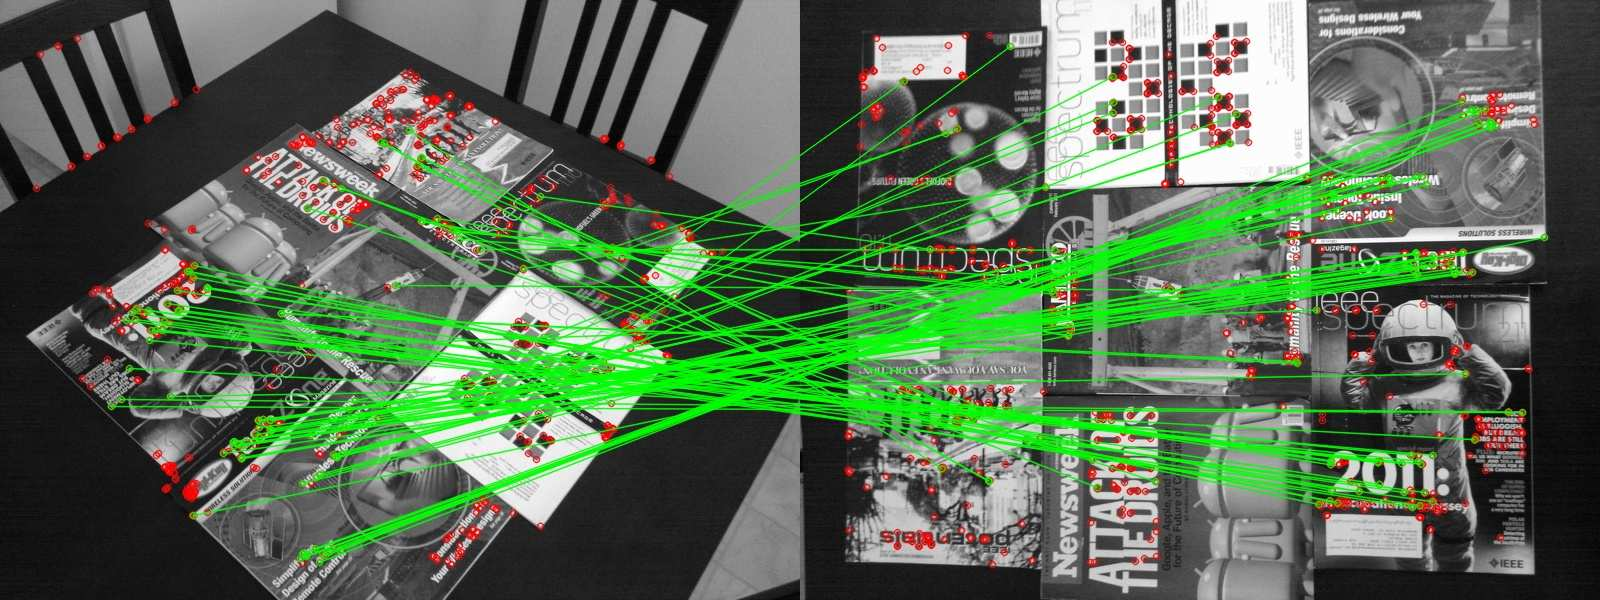
\includegraphics[width=0.8\textwidth]{orb-match}
	\caption{Divu attēlu atbilstošo raksturpunktu pāru noteikšana ar ORB~\cite{ORB}.}
	\label{fig:orb}
\end{figure}

Raksturpunktu pāru atrašanas ir atbilstošo punktu atrašana divos
(vai vairākos) attēlos, kuri atbilst vienam un tam pašam attēlā redzamam
objektam. Piemērs redzams \ref{fig:orb}~attēlā, kur ar zaļām līnijām
savienoti atrastie raksturpunktu pāri un ar sarkanu apzīmēti raksturpunkti,
kuriem pāris nav atrasts.

Raksturpunktu pāru noteikšana tiek izmantota tādos mašīnredzes pielietojumos, kā
% TODO: citēt pielietojumus
objektu atpazīšanā un sekošanā, attēlu ,,sašūšanā'', 
telpiskās informācijas rekonstrukcijā (kartēšanā) no attēliem,
vienlaicīgā pašlokalizācijā un kartēšanā (SLAM), u.c..

Raksturpunktu pāru noteikšanas pamatā ir šo punktu ,,aprakstīšana'' izveidojot
raksturpunkta \newTerm{deskriptoru}, kas satur informāciju,
kas ir pietiekami unikāla, lai nesakristu ar citiem raksturpunktiem attēlā
un ir noturīga pret sagaidāmām attēla īpašību izmaiņām, un to salāgošana
atrodot līdzīgos deskriptoru pārus.
Deskriptoram tātad nepieciešamas vai vēlamas šādas īpašības:
\begin{itemize}
	\item \newTerm{\emph{diskriminitāte}} --- spēja izšķirt raksturpunktus
		pēc to deskriptoriem;
	\item \emph{pozīcijas invariance} --- spēja salāgot raksturpunktus
		neatkarīgi no tā koordinātēm attēlā;
	\item \emph{rotācijas invariance} --- spēja salāgot raksturpunktus
		neatkarīgi no attēla rotācijas leņķa;
	\item \emph{intensitātes nobīdes invariance} --- spēja salāgot raksturpunktus
		neatkarīgi no globālas intensitātes izmaiņas;
	\item \emph{mēroga invariance} --- spēja salāgot raksturpunktus
		neatkarīgi no mēroga (attēla izmēru un/vai raksturpunkta objekta attāluma izmaiņa);
	\item \emph{perspektīvas invariance} --- spēja salāgot raksturpunktus
		neatkarīgi no perspektīvas (attēla uzņemšanas pozīcijas izmaiņa);
	\item \emph{trokšņu noturība} --- spēja salāgot raksturpunktus
		attēlā (iespējami) neatkarīgi no ,,trokšņa'' līmeņa attēlā;
\end{itemize}
Ir norādītas vairākas attēla izmaiņu invariances īpašības,
kas nozīmē, ka šī informācija nav izmantojama,
lai aprakstītu raksturpunktu.
Variance ir nepieciešama, lai nodrošinātu diskriminitāti un, praktiski visos
algoritmos, tiek izmantota lokālas intensitātes izmaiņas attēlā 
rakturpunkta tuvējā apkārtnē.

Eksistē vairāki algoritmi deskriptoru izgūšanai un
salīdzināšanai, t.sk.,~%
SIFT, % FIXME: Vai SIFT arī apzīmē deskriptoru?
SURF, BRIEF un tā varianti, ORB, u.c..
Algoritmus var izvērtēt pēc jau uzdotajām īpašībām, 
bet jāņem vērā arī to veiktspējas īpašības:
\begin{itemize}
	\item \emph{skaitļošanas kompleksitāte}, kas tieši ietekmē algoritma
		ātrdarbību;
	\item \emph{informācijas blīvums}, kas atspoguļo cik liela ir katra
		informācijas bita variance, kas ļauj sasniegt lielāku diskriminitāti
		pie mazāka bitu skaita.
\end{itemize}
% TODO?: Izvērst dažādo algoritmu teorētisko aprakstu?

Netiešs, bet būtisks, pāru noteikšanas ietekmējošais faktors ir 
labu raksturpunktu
atlase no attēla, jo salāgošana tiek veikta tikai starp atlasītajiem
punktiem. Raksturpunktu (un to detektēšanas algoritmu) galvenās īpašības
ir to variance, kas nosaka cik aprakstoši ir šie punkti,
un \newTerm{atkārtojamība}, kas izsaka atbilstošo punktu pāru piederību
raksturpunktu kopai dažādos attēlos pret kopējo raksturpunktu skaitu~%
\cite{FAST}\cite{SIFT-FPGA}.
Raksturpunktu atlases algoritmi un to īpašības plašāk apskatītas
\ref{sec:corners}~apakšnodaļā.

Šajā darbā, turpmākai algoritma implementāciju veiktspējas izvērtēšanai
un salīdzināšanai izvēlēts, ORB algoritms, vai konkrētāk tā salāgošanas
komponente --- rBRIEF.
% TODO: Forward ref
Šāda izvēle pamatota ar to, ka rBRIEF raksturpunktu salāgošanas
spēja ir līdzīga vai labāka nekā SIFT, bet ir par divām kārtām ātrāks nekā
SIFT un par kārtu ātrāks nekā SURF \cite{ORB}.
rBRIEF deskriptors ir arī noturīgāks pret troksni nekā
SIFT un tā rotācijas invariance līdzvērtīga SIFT \cite{ORB}.



\subsection{Attēlu raksturpunktu atlases algoritmi} \label{sec:corners}
Attēlu raksturpunktu atlase ir punktu apakškopas atlase pēc noteiktiem
kritērijiem. Kā jau minēts nodaļas ievadā (\pageref{sec:algo}~lpp.),
raksturpunktu atlasei bieži tiek izmantoti ,,stūru'' meklēšanas algoritmi,
kādi ir arī visi šajā darbā apskatītie raksturpunktu atlases algoritmi.

% TODO: Algoritmu aprakstošās īpašības

Eksistē vairāki stūru atrašanas algoritmi: \termEn{Harris} stūru detektors,
SUSAN, SIFT, KFT, FAST, u.c.. 
Šajā darbā apskatītais ORB algoritms, rakturpunktu atlasei izmanto oFAST, kas
ir FAST modifikācija, kas nosaka arī virziena informāciju.


	% TODO: Video apstrādes algoritmi
	
	
	%% Praktiskā daļa
	% TODO
	
	
	%% Literatūras saraksts
	\clearpage{\raggedright
	\begin{thebibliography}{99}
		\addcontentsline{toc}{section}{\refname}
		%~ \bibitem{VHSIC}
			%~ Creasey~D.J.,
			%~ \textit{Advanced Signal Processing}.\linebreak[1]
			%~ London: Peter~Peregrinus, 1985. ISBN~0-86341-037-5
		
		\bibitem{Fatahalian}
			Fatahalian~K., Houston~M.,
			``A Closer Look at GPUs.''\linebreak[1]
			\textit{Communications of the ACM} 51.10, pp.~50--57, 2008.
		
		\bibitem{Flynn-arch}
			%Michael J.~Flynn,
			Flynn~M.J.,
			\textit{Computer Architecture: Pipelined and Parallel Processor Design}.
			\linebreak[3]
			London: Jones~and~Bartlett, 1995. ISBN~0-86720-204-1
		
		\bibitem{Mokhtarian}
			Mokhtarian~F., Mohanna~F.,\linebreak[1]
			``Performance evaluation of corner detectors using
			consistency and accuracy measures.''
			\textit{Computer Vision and Image Understanding}~102, pp.~81--94, 2006.
		
		\bibitem{von-Neumann}
			John von Neumann,
			\textit{First Draft of a Report on the EDVAC}, (1945).\linebreak[2]
			Ed.~Godfrey~M.D., 2011.
		
		\bibitem{Owens-GPU}
			Owens~J.D., Houston~M., Luebke~D.,~et~al.,
			``GPU Computing.''\linebreak[1]
			\textit{Proceedings of the IEEE}~96.5, pp.~879--899,
			2008.
		
		\bibitem{Patterson2}
			Patterson~D.A., Hennessy~J.L.,\linebreak[1]
			\textit{Computer Architecture: A Quantitative Approach},
				5\nth ed..\linebreak[1]
			Waltham: Morgan~Kaufmann, 2012. ISBN~978-0-12-383872-8
		
		\bibitem{Patterson}
			Patterson~D.A., Hennessy~J.L., \linebreak[1]
			\textit{Computer Organization Design: %\linebreak[1]
				The Hardware/Software Interface}, 3\rd ed..\linebreak[1]
			San~Francisco: Morgan~Kaufmann, 2005. ISBN~1-55860-604-1
		
		\bibitem{Rosten-tracking}
			Rosten~E., Drummond~T.,\linebreak[1]
			``Fusing Points and Lines for High Performance Tracking.''\linebreak[1]
			\textit{IEEE International Conference on Computer Vision} vol.~2,
			pp.~1508--1511, 2005.
		
		\bibitem{FAST}
			Rosten~E., Drummond~T.,
			``Machine learning for high-speed corner detection.''
			\textit{European Conference on Computer Vision}, vol.~1, pp.~430--443,
			2006.
		
		\bibitem{ORB}
			Rublee~E., Rabaud~V., Konolige~K.,~et~al.,\linebreak[1]
			``ORB: an efficient alternative to SIFT or SURF.''\linebreak[1]
			\textit{IEEE International Conference on Computer Vision},
			pp.~2564--2571, 2011.
		
		\bibitem{Cache}
			Sorin~D.J., Hill~M.D., Wood~D.A.,
			\textit{A Primer on Memory Consistency and Coherence}.
			San~Rafael: Morgan~\&~Claypool, 2011. ISBN~978-1608455645
		
		\bibitem{SIMD}
			Stokes~J.,
			\textit{SIMD architectures} [online]. Ars Technica, 2000 %---
			[cites~April~16,~2014].\linebreak[1]
			Available: \url{http://arstechnica.com/features/2000/03/simd/}
		
		\bibitem{JIS}
			Šmēdiņš~J.,
			\textit{Iekļautās sistēmas mikrokontroliera kodola izstrāde}.\linebreak[1]
			Venstpils Augstskola, 2012.
		
		\bibitem{SIFT-FPGA}
			Tabib~W.,
			\textit{FPGA-Based Feature Detection}.
			Carnegie Mellon University, 2012.
		
		%~ \bibitem{Golshan-ASIC}
			%~ Golshan~K.,
			%~ \textit{Physical Design Essentials: An ASIC Design Implementation Perspective}.
			%~ New York: Springer, 2007. ISBN~0-387-36642-3
		
		%~ \bibitem{Heath}
			%~ %Steve Heath,
			%~ Heath~S.,
			%~ \textit{Embedded systems design}, 2\nd edition.\linebreak[3]
			%~ Oxford: Newnes, 2003. ISBN~0-7506-5541-1
		
		%~ \bibitem{VITAL}
			%~ IEEE,
			%~ \textit{IEEE 1076.4/D1, DRAFT Standard, VITAL ASIC Modeling Specification}.
			%~ New York: IEEE, 2000.
		
		%~ \bibitem{ieee-1364.1}
			%~ IEEE,
			%~ \textit{IEEE Std. 1364.1-2002, IEEE Standard for Verilog Register Transfer Level Synthesis}.
			%~ New York: IEEE, 2002.
		
		%~ \bibitem{HDL}
			%~ %Gaurav Mehta, Sridhar Kintali,
			%~ Mehta~G., Kintali~S.,
			%~ \textit{Hardware Description Languages}.\linebreak[2]
			%~ Santa Barbra: University of California,
			%~ 2009.
		
		
		%~ \bibitem{Perry-VHDL}
			%~ %Douglas L.~Perry,
			%~ Perry~D.L.,
			%~ \textit{VHDL: Programming by Example}, 4\nth edition. \linebreak[2]
			%~ New York: McGraw-Hill, 2002. ISBN~0-07-140070-2
		
		%~ \bibitem{Vivek-Verilog}
			%~ %Vivek Sagadeo,
			%~ Sagdeo~V.,
			%~ \textit{The Complete Verilog Book}.\linebreak[2]
			%~ Norwell: Kluwer Academic Publishers, 1998. ISBN~0-7923-8188-2
		
		%~ \bibitem{Vahid-RTL}
			%~ %Frank Vahid,
			%~ Vahid~F.,
			%~ \textit{Digital Design with RTL Design, VHDL, and Verilog}, 2\nd edition.\linebreak[2]
			%~ New York: % Hell knows which city
			%~ John Wiley \& Sons, 2011. ISBN~978-0-470-53108-2
		
		%~ \bibitem{FusionGuide}
			%~ Actel corp.,
			%~ \textit{Fusion Embedded Development Kit User's Guide}. %\linebreak[2]
			%~ %USA: Actel,
			%~ 2009.
		
		%~ \bibitem{FlashROM}
			%~ Actel corp.,
			%~ \textit{Fusion FlashROM}, Application Note AC236. %\linebreak[2]
			%~ %USA: Actel,
			%~ 2005.
		
		%~ \bibitem{RAM4K9}
			%~ Actel corp.,
			%~ \textit{Fusion SRAM/FIFO Blocks}, Application Note AC237. %\linebreak[2]
			%~ %USA: Actel,
			%~ 2005.
		
		%~ \bibitem{FusionFAQ}
			%~ Actel corp.,
			%~ \textit{Synplify — Synthesis Frequently Asked Questions}. %\linebreak[2]
			%~ %USA: Actel,
			%~ 2009.
		
		%~ \bibitem{SmartFusionFabric}
			%~ Microsemi corp.,
			%~ \textit{SmartFusion FPGA Fabric User's Guide}.
			%~ %USA: Microsemi,
			%~ 2011.
		
		%~ \bibitem{Xilinx7}
			%~ Xilinx,
			%~ \textit{7 Series FPGAs Overview}.
			%~ %USA: Xilinx,
			%~ 2012.
		
		%~ \bibitem{Mealy-VHDL}
			%~ %Bryan Mealy, Fabrizio Tappero,
			%~ Mealy~B., Tappero~F.,
			%~ \textit{Free Range VHDL}.
			%~ 2012. [tiešsaiste] \linebreak[2]
			%~ Pieejams: \url{http://www.freerangefactory.org/dl/free_range_vhdl.pdf}\linebreak[2]
			%~ \mbox{[skatīts on 2012.~gada 2.~maijā]}
		
		%~ \bibitem{vhdl-vs-verilog}
			%~ Smith~D.J.,
			%~ \textit{VHDL \& Verilog Compared \& Contrasted}. [tiešsaiste]\linebreak[2]
			%~ Pieejams: \url{http://www.angelfire.com/in/rajesh52/verilogvhdl.html}
			%~ \mbox{[skatīts on 2012.~gada 21.~maijā]}
		
		%~ \bibitem{Kumar-Verilog}
			%~ % Deepak Kumar Tala,
			%~ Tala~D.K., \textit{Gate Level Modeling}. [tiešsaiste]\linebreak[2]
			%~ Pieejams: \url{http://www.asic-world.com/verilog/gate.html}
			%~ \mbox{[skatīts on 2012.~gada 24.~maijā]}
	\end{thebibliography}
} % "End of \raggedright"

	
\end{document}
